
\documentclass{article}
\usepackage{graphicx}
\usepackage{enumerate}
\usepackage{xcolor}
\usepackage[colorlinks]{hyperref}
\RequirePackage{amsmath,amssymb}
\RequirePackage{xcolor,graphicx}
\RequirePackage{tikz,pgfplots}
\usetikzlibrary{shapes,arrows,positioning,matrix,backgrounds,fit}



\begin{document}

\title{Rising Coders - Progress Tracker}
\author{170050067(40\%), 170050085(30\%), 170050053(30\%)}
\maketitle
\renewcommand\abstractname{Declaration}
\begin{abstract}
Here is the text of your introduction.I acknowledge and understand that plagiarism is wrong. This project is my own work, or my group’s own unique group project. I acknowledge that copying some-
one else’s work, or part of it, is wrong, and that submitting identical work to others
constitutes a form of plagiarism.
\end{abstract}
\section{Work Done so far}


\section{System Architecture using TikZ}

\bigskip

\scalebox{2}{
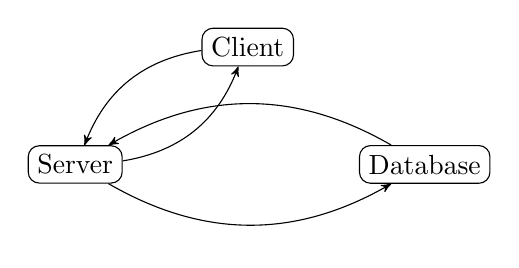
\begin{tikzpicture}
[->,>=stealth',auto,node distance=3cm, main node/.style={draw,font=\sffamily\Large\bfseries}]

  \node (server) [rounded corners, draw=black] {Server};
  \node  (client) [rounded corners,above right =1cm and 1cm of server, draw=black]  {Client};
  \node (database) [rounded corners, right =3cm of server , draw=black] {Database};
  \path  [every node/.style={font=\sffamily\small}]
  (client) edge [bend right] node [left] {} (server)
  (server) edge  [bend right] node [left] {} (client)
  (server) edge [bend right] node [right] {} (database)
  (database) edge[bend right] node [left] {} (server);
  
\end{tikzpicture} }

\bigskip

\section{Results and Analysis}
\begin{figure}[ht]
\graphicspath{ {/home/} }
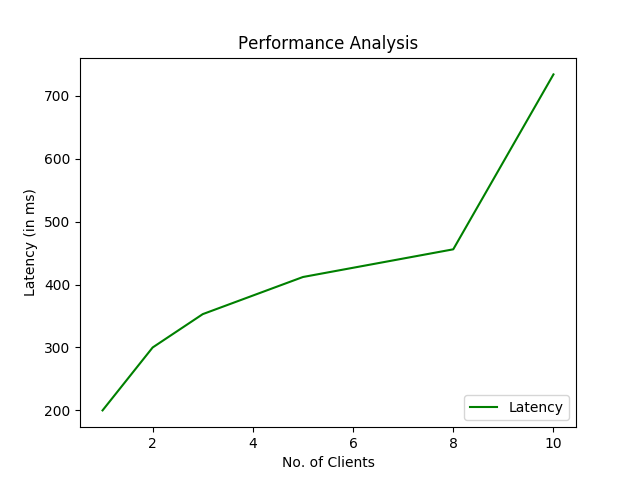
\includegraphics{PerformanceAnalysis}
\end{figure}
\begin{figure}[h]
\graphicspath{ {/home/} }
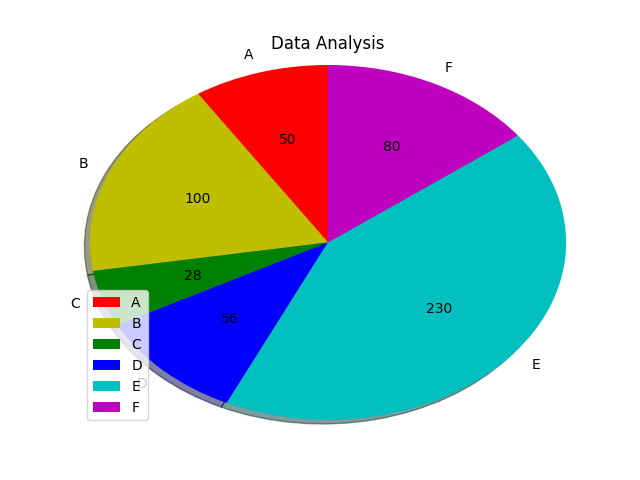
\includegraphics{DataAnalysis}

\end{figure}




\section{Future Work}


\section*{References}
\begin{enumerate}%for capital roman numbers.
\item [][1] Inspired from Google, available at \href{http://google.co.in}{\color{blue}http://google.co.in.}
\item [][2] For more information about ’TikZ’, click here: \href {https://tex.stackexchange.com/?tags=tikz-pgf}{\color{blue}TikZ}
\end{enumerate}

\end{document}
